\begin{frame}{Probing Model}

To theoretically evaluate the security, we consider the probing model \cite{C:IshSahWag03}.
\pause
\begin{itemize}
	\item The $t$-probing model assumes that an adversary is able to peek any $t$ intermediate values in the algorithm.
	\pause
	\item To be secure in the $t$-probing model ($t$-probing secure), $n \geq t+1$.
	\pause
	\item It is complicated to prove $t$-probing security directly, so we apply the concept of \emph{non-interference security}.
\end{itemize}

\end{frame}


\begin{frame}{Non-Interference Security}

\begin{definition}{$t$-Non-Interference ($t$-NI) Security (from \cite{CCS:BBDFGS16})}
A gadget is $t$-Non-Interference ($t$-NI) secure if every set of $t$ intermediate values can be simulated by no more than $t$ shares of each of its inputs.
\end{definition}
\medskip
\pause

\begin{definition}{$t$-Strong Non-Interference ($t$-SNI) Security (from \cite{CCS:BBDFGS16})}
A gadget is $t$-Strong-Non-Interference ($t$-SNI) secure if for every set of $t_I$ internal intermediate values and $t_O$ of its output shares with $t_I + t_O \leq t$, they can be simulated by no more than $t_I$ shares of each of its inputs.
\end{definition}
\medskip

\hyperlink{sec:appendix-tni}{\color{blue}Appendix - Examples of Non-Interference Security}

\end{frame}


\begin{frame}{Non-Interference Security}

\begin{columns}[T]

\begin{column}{0.5\textwidth}

Takeaway:
\visible<2->{
\begin{itemize}
	
	\item If a gadget is $t$-(S)NI secure for $t=n-1$, and if any $n-1$ input shares are independent to the secret, then the gadget is $t$-probing secure.
	
	\visible<3->{\item $t$-SNI is stronger than $t$-NI by definition.}
	
	\visible<5->{\item A composition of $t$-NI gadgets may not be $t$-NI, so we insert $t$-SNI gadgets to make it $t$-NI or $t$-SNI.}
\end{itemize}
}
\end{column}

\begin{column}{0.4\textwidth}
\visible<4->{
	\begin{figure}
	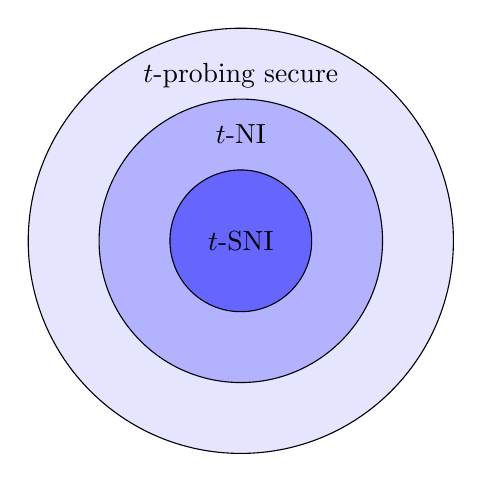
\begin{tikzpicture}[node distance=1cm]

	\draw[fill = blue!10!white] (0,0) circle (2.7) node [black, yshift=2.1cm] {$t$-probing secure};
	\draw[fill = blue!30!white] (0,0) circle (1.8) node [black, yshift=1.35cm] {$t$-NI};
	\draw[fill = blue!60!white] (0,0) circle (0.9) node [black] {$t$-SNI};

	\end{tikzpicture}
	\end{figure}
}    
\end{column}

\end{columns}

\end{frame}


\begin{frame}{Gadgets in Our Work}

\begin{table}
\centering
	\begin{tabular}{l l | l l} 
	\toprule
	\textbf{Algorithm} & \textbf{Security$\quad$} & \textbf{Algorithm} & \textbf{Security$\quad$} \\
	\midrule
	{\sf SecAnd} & $t$-SNI & {\sf SecOr} & $t$-SNI \\
	{\sf SecMult} & $t$-SNI & {\sf SecNonzero} & $t$-SNI \\
	{\sf SecAdd} & $t$-NI & {\sf SecFprUrsh} & $t$-SNI \\
	{\sf A2B} & $t$-SNI & {\sf SecFprNorm64} & $t$-NI\\
	{\sf B2A} & $t$-SNI & {\sf SecFPR} & $t$-SNI \\
	${\sf B2A_{Bit}}$ & $t$-SNI & {\sf SecFprMul} & $t$-SNI\\
	{\sf RefreshMasks} & $t$-NI & {\sf SecFprAdd} & $t$-SNI\\
	{\sf Refresh} & $t$-SNI \\
	\bottomrule
	\end{tabular}
\caption{List of gadgets/algorithms in our work with $n=t+1$ shares}
\label{table:gadgets_secureity}
\end{table}
\end{frame}



\begin{frame}{Test Vector Leakage Assessment (TVLA)}

For practical security validation, we apply the Test Vector Leakage Assessment (TVLA) \cite{gilbert2011testing}.
\pause

\begin{columns}

\begin{column}{0.5\textwidth}

A tester records two sets of traces where
\pause

\begin{itemize}
	\item Set 1: fixed input
	\pause
	\item Set 2: random inputs
\end{itemize}
\pause

The Welch's $t$-test is then applied.

\end{column}

\pause

\begin{column}{0.4\textwidth}

\[ 
	t = \frac{ \bar{x}_f - \bar{x}_r }{ \sqrt{ \frac{s_f^2}{n_f} + \frac{s_r^2}{n_r} } }
\]

\begin{itemize}
	\item $\bar{x}_f, \bar{x}_r$: Sample means.
	
	\item $s_f^2, s_r^2$: Sample variances.

	\item $n_f, n_r$: Sample sizes.
\end{itemize}

\end{column}

\end{columns}
\pause
\medskip
\medskip

By convention, the leakage is significant if the $t$-value exceeds $\pm 4.5$.

\end{frame}
